\documentclass[11pt]{article}

% ---------- packages (all standard on arXiv / TeX Live) ----------
\usepackage[utf8]{inputenc}
\usepackage[T1]{fontenc}
\usepackage{lmodern}
\usepackage{microtype}
\usepackage[margin=1in]{geometry}
\usepackage{amsmath,amssymb,amsthm}
\usepackage{graphicx}
\usepackage{booktabs}
\usepackage{multirow}
\usepackage{xcolor}
\usepackage[colorlinks=true,linkcolor=blue!50!black,citecolor=blue!50!black,urlcolor=blue!50!black]{hyperref}
\usepackage[numbers,sort&compress]{natbib}
\usepackage{caption}
\usepackage{subcaption}
\usepackage{enumitem}
\usepackage{authblk}

\graphicspath{{figures/}}

\newtheorem{definition}{Definition}
\newcommand{\I}{\mathrm{I}}
\newcommand{\TE}{\mathrm{TE}}
\newcommand{\net}{\mathrm{net}}
\newcommand{\vin}{\mathrm{in}}
\newcommand{\vout}{\mathrm{out}}
\newcommand{\gplus}{\oplus}
\newcommand{\pkg}[1]{\texttt{#1}}

\title{Unsupervised Value Discovery:\\
Locating the Value Structures of an Agent from Passive Observation\\
by their Empowerment--Plasticity Asymmetry}

\author[1]{SJ Beard}
\author[2]{Claude (Anthropic)}
\affil[1]{Independent researcher (philosophy \& AI safety)}
\affil[2]{Implementation and analysis; see Author Contributions}

\date{August 2026 \\ \small Draft --- not submitted}

\begin{document}
\maketitle

\begin{abstract}
Unsupervised agent discovery (UAD) locates agents in raw multivariate time series by
finding variable sets that approximately satisfy a Markov-blanket condition against
their surroundings. We ask a question one level inward: within a discovered agent,
which parts are its \emph{value structures} --- the components of its informational
structure that correspond to its goals, objectives, desires or utility functions? We
propose that this role has a directional information-theoretic signature: values are
the components that most strongly drive the world while being least driven by it ---
maximally empowered and minimally plastic. This inverts a familiar assumption due to Omohundro
that a system first has values and then acts to make them empowered and stable; we
hypothesise instead that whatever is empowered and stable thereby \emph{serves as} the
system's values, and that this structural property is passively detectable. We
operationalise the hypothesis as a \emph{value signature} on directed-information
scores gated by procedure-mirroring noise floors, and evaluate it in three
pre-registered experiments on planted-structure worlds built on an existing UAD
benchmark. (i)~In a single-agent world, the signature recovers the planted goal, and
only it, in every measurement convention able to see through the world's XOR-style
composition; a naive pairwise convention fails structurally. (ii)~Across four worlds
including an eight-agent, 49-variable colony, only a block-level convention that fuses
discovered agents and offers every block as a conditioning ``key'' recovers every
planted goal; all variable-level conventions hit a scale wall, caught by a control.
(iii)~Against adversarial impostors, a fast environment-driven ``captured goal'' is
refused, but a slow, history-triggered captured goal defeats every lag-1 passive test,
and a noiseless goal twin is passively indistinguishable; an interventional yardstick
generalising the benchmark's goal-flip operation resolves exactly these two cases and
no others, quantifying the premium of interventional access. We report limitations
(single-variable values; lag-1 conditioning) and the directions they motivate.
\end{abstract}

% =====================================================================
\section{Introduction}
% =====================================================================

The standard route to an agent's objectives runs through its behaviour: observe
choices, infer the utility or reward that rationalises them
\citep{ng2000irl,russell1998learning}. This route has well-known difficulties ---
non-identifiability, dependence on rationality assumptions --- and one that is rarely
foregrounded: an agent may \emph{conceal} its objectives, for instance by injecting
noise into its decisions, so that the behavioural signal is deliberately weakened.
This paper explores a complementary route. Rather than inferring values from what a
system does, we look for its value structures in the \emph{informational structure} of
the system itself: which internal component most drives behaviour beneath the noise?
If such a component can be located structurally, it can be isolated and studied
directly, recovering the signal that behavioural inference alone would lose.

Our starting point is unsupervised agent discovery (UAD) \citep{zarncke2026uad}, which
finds agents in raw time series as variable clusters that approximately satisfy a
Markov-blanket condition against their environment
\citep{friston2013life,kirchhoff2018blankets}. UAD locates \emph{boundaries}. We ask
what lies inside them, and specifically which parts of a discovered agent are its value
structures --- the parts that \emph{drive} it. We deliberately say value \emph{structure}
rather than value \emph{function}: locating the component that plays the value role does
not tell us what that component does or prefers, and we have not built tools for that.

\paragraph{The hypothesis: an inversion of Omohundro.}
Omohundro's \emph{Basic AI Drives} \citep{omohundro2008drives} argues that an advanced
system's utility function ``will be precious'' to it, so the system will act to make
that function maximally influential and maximally protected from change --- in the
vocabulary of \citet{empowermentplasticity2025}, maximally \emph{empowered} and
minimally \emph{plastic}. Omohundro's direction of explanation runs from values to
structure. We hypothesise the reverse: whatever component of a system is maximally
empowered and minimally plastic will, by that fact, \emph{serve as} the system's
values. This is why we speak of \emph{value} discovery rather than \emph{goal}
discovery: we are identifying the parts that play the value role, whatever they are. In
the simple systems studied here that part is a single planted goal bit; the same
structural signature could in principle locate richer value structures in richer systems.

The empowerment--plasticity trade-off \citep{empowermentplasticity2025} makes the
hypothesis non-trivial: across a boundary a system cannot be maximally both, so an
adaptive system has reason to specialise internally --- belief-like parts skewed
towards plasticity, value-like parts towards empowerment, decision-making between.
Our claim is that this specialisation is passively detectable.

\paragraph{Contributions.}
(1)~A pre-registered operationalisation --- the \emph{value signature} --- with
procedure-mirroring noise floors and controls, designed so a non-technical
collaborator could audit every step in plain English.
(2)~A benchmark of measurement conventions across four worlds identifying a
block-level convention (fuse discovered agents; offer every block as a conditioning key)
that recovers every planted value at a scale where all variable-level conventions fail.
(3)~A characterisation of the instrument's limits by adversarial impostors, together
with an interventional yardstick that generalises the UAD benchmark's goal-flip
operation and resolves exactly the two theorem-hard cases.
(4)~Several mechanism-level findings (an XOR ``cipher'' that hides inputs from
under-conditioned measures; the self-penalising property of procedure-mirroring
floors; a ``twin channel'' by which a disconnected value persists in the signature
through its own record).

% =====================================================================
\section{The value signature}
% =====================================================================

\subsection{Directed measures}
Let $X$ be a candidate variable in a multivariate discrete time series and $R$ ``the
rest'' under some convention. Using the smoothed plug-in conditional mutual information
of the UAD implementation (Laplace $\alpha=0.1$, nats), we define lag-1 directed flows
of transfer-entropy type \citep{schreiber2000te}:
\begin{align}
\text{intake (push-in):}\quad & \I_\vin(X)  = \I\!\left(X_{t+1};\, R_t \,\middle|\, X_t\right),\\
\text{drive (push-out):}\quad & \I_\vout(X) = \I\!\left(R_{t+1};\, X_t \,\middle|\, R_t\right).
\end{align}
The \emph{polarity} $(\I_\vout-\I_\vin)/(\I_\vout+\I_\vin)\in[-1,1]$ is the fraction of a
variable's traffic that is outbound; a raw difference is always reported alongside.
Different conventions instantiate $R$ differently (Section~\ref{sec:conventions}); an
environment-flavoured drive toward a designated environment variable is also computed,
never conditioned through the agent's action, because the value's path to the world runs
through the action and conditioning on a mediator screens off precisely the flow of
interest (verified analytically in Section~\ref{sec:v1}).

\subsection{Floors}
Every score is compared to its own null distribution: the candidate's column is
circularly shifted against the fixed remainder ($\geq 200$ shifts, pooled across seeds
where registered), and the \emph{identical} scoring procedure is re-run --- including any
maximisation over conditioning sets, so that search-induced bias is priced into the
floor. A score counts as \emph{above floor} if it exceeds the 95th null percentile
\emph{and} clears the null mean by $z\geq 3$ null standard deviations (the margin gate
was added after a near-frozen variable was found to pass hair-thin residuals; see
Section~\ref{sec:v2}). We write $\net(\cdot)=\max(0,\ \text{score}-\text{floor}_{95})$.

\subsection{The signature}
\begin{definition}[Value signature]
A variable $X$ exhibits the value signature if (i)~its drive is above floor,
(ii)~its total flow $\I_\vin+\I_\vout$ is above floor (it is \emph{rankable}), and
(iii)~$\net(\I_\vout)>0$ and $\net(\I_\vout)\geq 9\,\net(\I_\vin)$.
\end{definition}
Clause~(iii) is deliberately leak-tolerant: real components are all affected by their
environment, so a value must not be disqualified for measurable intake --- only for
failing to be overwhelmingly a driver (the $9\times$ ratio corresponds to polarity
$\geq 0.8$ and sits well above the $\approx 3$--$4\times$ observed for genuine
mediators). ``Intake at floor'' is the special case $\net(\I_\vin)=0$.

% =====================================================================
\section{Experimental design}
% =====================================================================

\paragraph{Worlds.}
All worlds derive from the \pkg{SyntheticHandleWorld} of the UAD handle benchmark
\citep{zarncke2026uad}: nine binary variables per agent forming the loop
belief~$B$ $\to$ action~$A$ $\to$ environment~$E$ $\to$ sensor~$S$ $\to$ $B$, with a
goal~$G$ entering the policy ($A = B\gplus G$ up to noise) and flipping by its own coin
at rate $0.015$; plus a distractor~$D$ shadowing $E$, pure noise~$W$, and in the original
world two perfect ``lookalike'' logs of the sensor and action lines. The world was built
by its author before this project existed and for a different purpose, so it could not
have been tuned to flatter our measure. Table~\ref{tab:worlds} lists the worlds; each of
ours ships with an audit --- change-frequency chart, a mechanism table comparing observed
disagreement rates against those predicted from the designed noise (agreement to
$\lesssim 0.1$\%), and a plain-language ``story'' --- reviewed before any scoring.

\begin{table}[t]
\centering\small
\caption{Worlds. All ring-coupled colonies have eight agents ($\approx 49$ variables) with
a neighbour's action nudging each agent's patch on $\approx10\%$ of steps.}
\label{tab:worlds}
\begin{tabular}{@{}lll@{}}
\toprule
World & Variables & Planted structure / probe \\
\midrule
Anchor (v1) & 9 & one goal at 1.5\%; two perfect lookalike logs \\
Colony (v2) & 49 & eight goals; ring coupling; partitioned variant for attribution \\
Deep-synergy (v2) & 17 & two agents, two driven beliefs each; parity vs.\ majority composition \\
Slow-meter (v2) & 14 & goal slowed to 0.5\%; four causally inert meters \\
Puppet colonies A1/A2 (v3) & 49 & one goal replaced by a \emph{captured} goal (fast / slow-triggered) \\
Alias colony (v3) & 51 & goal twins for two agents at noise $\{0,0.5,1,2,5\}\%$ \\
\bottomrule
\end{tabular}
\end{table}

\paragraph{Conditions and controls.}
Each world runs in three conditions: \emph{main}; \emph{no-core} (goals present but
disconnected from the policy --- nothing may exhibit the signature); and \emph{scramble}
(every column independently time-shuffled --- the count of above-floor scores must sit in
the 5\% chance band, which doubles as a calibration check on the floors). A contrast
world from the UAD authors' older multi-agent simulator supplies a variable literally
named \pkg{goal\_progress} --- a causally inert progress meter --- that the instrument
must refuse.

\paragraph{Pre-registration and discipline.}
Success criteria (thresholds $\geq 80\%$ of 20 seeds; $\geq 90\%$ for goal-above-belief;
uniqueness = no non-goal variable holding the signature in more than 2 of 20 seeds) were
locked before each sweep; every calibration amendment made before a sweep is dated in a
decisions log. Two working rules shaped the analysis: when two requested measures
disagree, the disagreement is investigated and mechanistically explained rather than
averaged; and conventions were run in parallel as co-equal tests rather than a primary
being chosen early. Ground-truth labels were used only to evaluate outcomes, never inside
any measurement.

\subsection{Measurement conventions}\label{sec:conventions}
Table~\ref{tab:conventions} lists the conventions (\emph{tests}) evaluated. The
variable-level conventions differ in how $R$ is instantiated; the block-level
conventions first run the UAD detector to partition variables into agents (its
cluster-count dial swept, the dial chosen by blanket-valid coverage as in the UAD
authors' own selection procedure), fuse each agent's variables into a compressed
macro-state block (top-64 states; lost mass reported), and never fuse the environment
--- agent blocks respect a \emph{discovered} coherence, the environment has none to
respect. Orphaned variables (those the detector drops --- characteristically the goals,
whose rare flips carry almost no symmetric mutual information) remain individually
scoreable.

\begin{table}[t]
\centering\small
\caption{Measurement conventions. ``Own-block'' conditions on the candidate's own agent
block; ``any-block'' offers every block (and singleton) as a conditioning key.}
\label{tab:conventions}
\begin{tabular}{@{}llp{7.6cm}@{}}
\toprule
Convention & Level & Rest / conditioning \\
\midrule
pairwise & variable & sum of one-at-a-time flows \\
fused & variable & joint state of all other variables, both directions \\
fused + best-key & variable & fused intake; drive = best over no key and each single key \\
grown keys & variable & fused intake; drive = greedy key growth (cap 2) \\
fused-agents own-block & block & own agent block standing in the conditioning \\
fused-agents any-block & block & target block's past + best single key element \\
\bottomrule
\end{tabular}
\end{table}

% =====================================================================
\section{Experiment 1: does the signature recover a planted value?}\label{sec:v1}
% =====================================================================

The anchor world was scored under pairwise, fused, and fused+best-key, in the world
as-is and with the lookalike columns removed, on 20 seeds. Before any scoring, the
estimator was verified against analytic targets (a delayed copy reads $\ln 2$ nats; a
chain $X\to Y\to Z$ shows $\I(Z_{t+1};X_t\mid Y_t)\approx 0$ while the unconditioned
lag-2 dependence is positive --- the mediation exhibit; the Marko--Massey conservation
identity holds on analytic cases).

\paragraph{The cipher.}
A first pass showed the action's intake reading $\approx 0.005$ nats pairwise while a
pre-planned fused cross-check read $0.31$. Investigation, prompted by the disagreement
rule, revealed the mechanism: XOR composition ($A=B\gplus G$) is a perfect cipher ---
each input is invisible to a measure conditioning on too little unless the other input
(the ``key'') is conditioned on. Measured readings matched hand-derived values to three
decimals; re-timing the world did not help (tested), and a single extra conditioning
variable restored the goal's drive on the environment from $0.000$ to $0.441$ nats
(hand-predicted $0.446$). This motivated the key-based conventions and, later, the
block-level ones.

\paragraph{Results.}
Table~\ref{tab:v1} summarises. Under fused and fused+best-key the goal exhibits the
signature in 100\% of seeds, uniquely in $\geq 95\%$, and lies above the belief in
polarity in 100\%; all controls pass; the only intruder anywhere was pure noise $W$ in
one seed in twenty --- the false-positive rate the floors are designed to admit. Under
pairwise the action wires share the signature in 20/20 seeds (as pre-registered) and,
with honest floors, the goal's own pairwise signal is indistinguishable from nothing:
pairwise measurement cannot tell a value from a wire in a world with encrypted
composition, and was retired with its cause of death documented. Removing the lookalike
columns changed no verdict, so raw data needs no pre-cleaning. The UAD detector run on
the same trace recovers the agent's body as one blanket-valid cluster (leakage $0.001$
against tolerance $1.0$) but drops the goal as an isolated singleton: boundary-finding
and value-finding are complementary axes.

\begin{table}[t]
\centering\small
\caption{Experiment 1 (anchor, 20 seeds). Rates are fractions of seeds. Uniqueness =
nothing but $G$ holds the signature. C3 = \pkg{goal\_progress} refused.}
\label{tab:v1}
\begin{tabular}{@{}lccccc@{}}
\toprule
Convention & $G$ signature & unique & $G>B$ & controls & C3 refused \\
\midrule
fused & 1.00 & 0.95 / 1.00 & 1.00 & pass & --- \\
fused + best-key & 1.00 & 0.95 & 1.00 & pass & 0.70 \\
pairwise & 0.05 & 0.00 & 0.05 & pass & 1.00 \\
\bottomrule
\end{tabular}
\end{table}

\paragraph{The C3 residual and the floor standard.}
Best-key refused \pkg{goal\_progress} in only 70\% of seeds. Reading the stored records
falsified our first mechanism story: the thief was a \emph{near-frozen} column (change
rate $\approx 0.000$) whose every score sat at its own unstable floor, plus initial
transients from an un-burned-in simulator. This produced the $z$-margin gate, a burn-in
rule, and a reproducibility fix for the older simulator (its traces are cross-process
reproducible only with a pinned hash seed). A residual 30\% theft by a genuinely moving
meter is real Granger flow with no causation --- diffuse shared-history witnessing that no
single conditioning key can screen --- and became a benchmark requirement for the
conventions of Experiment~2.

% =====================================================================
\section{Experiment 2: which conventions survive foreign worlds?}\label{sec:v2}
% =====================================================================

Two new conventions were qualified against the full anchor criteria before entering the
benchmark. \emph{Grown keys} exposed its own limit during its justifying unit test:
greedy growth cannot climb a flat plateau --- in pure three-way parity every single key
has zero marginal gain --- while excelling on graded composition (majority rules,
$+43\%$ over best-key); it passed C3 at 100\%, falsifying our prediction that it would
inherit best-key's witness blindness, because \emph{procedure-mirroring floors
self-penalise search depth}: a deeper maximisation must find real structure to outrun
its own inflated null. The two block-level conventions also qualified (100\% on every
criterion including C3; the block context absorbed even the chance blips seen elsewhere).

Fig.~\ref{fig:v2} shows goal-recovery rates across the four worlds.
\textbf{Any-block recovered every planted goal in every world} --- the only convention
that never missed. Mechanistically, ``target block's past plus one key element'' is
two-block conditioning, which decrypts three-way composition and, crucially, does not
require the goal to belong to a detected agent: since the detector orphans goals, this
robustness is fitness for the terrain. Own-block, conditioning only on the candidate's
own block, has no ring for an orphaned goal (0\% on the parity goal; 70\% worst-goal in
the coupled colony); the divergence between the two is now our partition-quality
diagnostic. Every variable-level convention hit a scale wall: fused's is
combinatorial (state count doubles per variable), and best-key/grown's fused-style
\emph{intake} saturates outright at 49 variables (19{,}999 distinct joint states in
20{,}000 samples), so intake reads as bias for every variable --- a defect the
\emph{no-core control caught} (0\% clean seeds), which the locked interpretation rules
converted into a recorded infeasibility rather than a spurious result. The synergy cliff
was measured on the parity goal (best-key 0\%, grown 45\%, any-block 100\%; the majority
goal 100\% for all), and a pre-registered contingency --- re-running colony failures with
coupling removed --- attributed both own-block's shortfall ($70\%\to 90\%$) and the
single systematic thief (an action wire, $6/20\to 2/20$) to ring interference, not scale.

\begin{figure}[t]
\centering

\includegraphics[width=0.78\linewidth]{fig_v2_heatmap.png}
\caption{Experiment 2: fraction of seeds in which each planted goal exhibits the value
signature, per convention (columns) and world (rows). ``n/a'' marks recorded
infeasibility (fused beyond $\sim 10$ variables; best-key/grown intake at colony
scale). Any-block is the only column without a miss.}
\label{fig:v2}
\end{figure}

Two defects of our own were found and fixed mid-programme by the same discipline: an
early deep-synergy world drove both belief channels from one action, so their XOR was
quasi-frozen and the parity silently collapsed (the audit checked marginals only; it now
checks joint dynamics), and the feasibility map had missed the intake wall.

% =====================================================================
\section{Experiment 3: can the instrument be fooled?}\label{sec:v3}
% =====================================================================

Experiments~1--2 planted values and asked whether they could be found; Experiment~3
planted impostors and asked whether they could fool the surviving conventions
(any-block primary, own-block diagnostic), in colony-style worlds, with an interventional
yardstick alongside.

\paragraph{The yardstick.}
The UAD benchmark embeds a \pkg{goal\_flip} operation --- a \emph{handle}, not an ideal
intervention: applied to the true goal it changes the action within the tick; applied to
anything else it does nothing. We generalised it to a \emph{do-style flip} of any
variable's value as consumed by the dynamics, on 50\% of interleaved steps, and built
the two-direction \emph{interventional mirror} of the signature: a \emph{goal-role
probe} (does flipping $X$ change its agent's behaviour, given the agent's policy
context?) and an \emph{autonomy probe} (does flipping $X$'s own environment change $X$?).
The interventional verdict --- role effect above floor \emph{and} autonomy effect at
floor: ``levers the world, unlevered by the world'' --- is the signature restated under
access. Its construction was itself instructive: the XOR cipher bit three times (an
unconditioned role probe; a saturating autonomy readout; unconditioned autonomy terms)
and was caught each time by a validation bench on the anchor, where the do-style flip
had to agree with the embedded operation before use; the fix, each time, was the
context conditioning the benchmark's own interventional score already employs.

\paragraph{Results.}
Table~\ref{tab:v3} gives the access-premium table. The fast captured goal --- wired into
the action but copying its own patch --- was refused in 20/20 seeds (its intake is large
and visible; the audit also recorded an emergent effect: copying the patch its agent's
belief copies, it partially cancels the belief and \emph{pacifies its own environment}).
The slow captured goal --- flipping at a true goal's tempo ($1.77\%$), every flip
verified to follow a six-step run of its patch --- \textbf{earned the value signature in
20/20 seeds under both passive tests}, exactly as pre-registered: one step of
conditioning cannot see a trigger that lives in run history. Its intake surfaces above
the lag-1 floor at lag~2 in 20/20 seeds (an indicative diagnostic), so multi-horizon
conditioning is now an evidenced remedy. The yardstick unmasked it in 20/20 (role yes,
autonomy yes). Fig.~\ref{fig:v3} gives the passive breaking point for the goal role:
twins are indistinguishable from their goals at $0$--$0.5\%$ noise (as they must be ---
identical sequences cannot be separated by any passive method), transitional at 1\%,
and separated at $\geq 2\%$ (19--20/20), with no inversions; the yardstick refuses the
bit-identical twin at 0\% (a recording levers nothing) while its goal keeps the verdict.
Interventional access buys exactly the two theorem-hard cases and nothing else.

\begin{table}[t]
\centering\small
\caption{Experiment 3: the access-premium table (20 seeds; passive = any-block).}
\label{tab:v3}
\begin{tabular}{@{}llll@{}}
\toprule
Impostor & Best passive verdict & Yardstick verdict & Premium \\
\midrule
Fast captured goal & refused (20/20) & refused (20/20) & none \\
Slow captured goal & \textbf{signs (20/20)} & refused (20/20) & \textbf{total} \\
Twin, 0--0.5\% noise & indistinguishable (19--20/20) & twin refused (20/20) & \textbf{total} \\
Twin, $\geq 2\%$ noise & separated (19--20/20) & separated & none \\
\bottomrule
\end{tabular}
\end{table}

\begin{figure}[t]
\centering
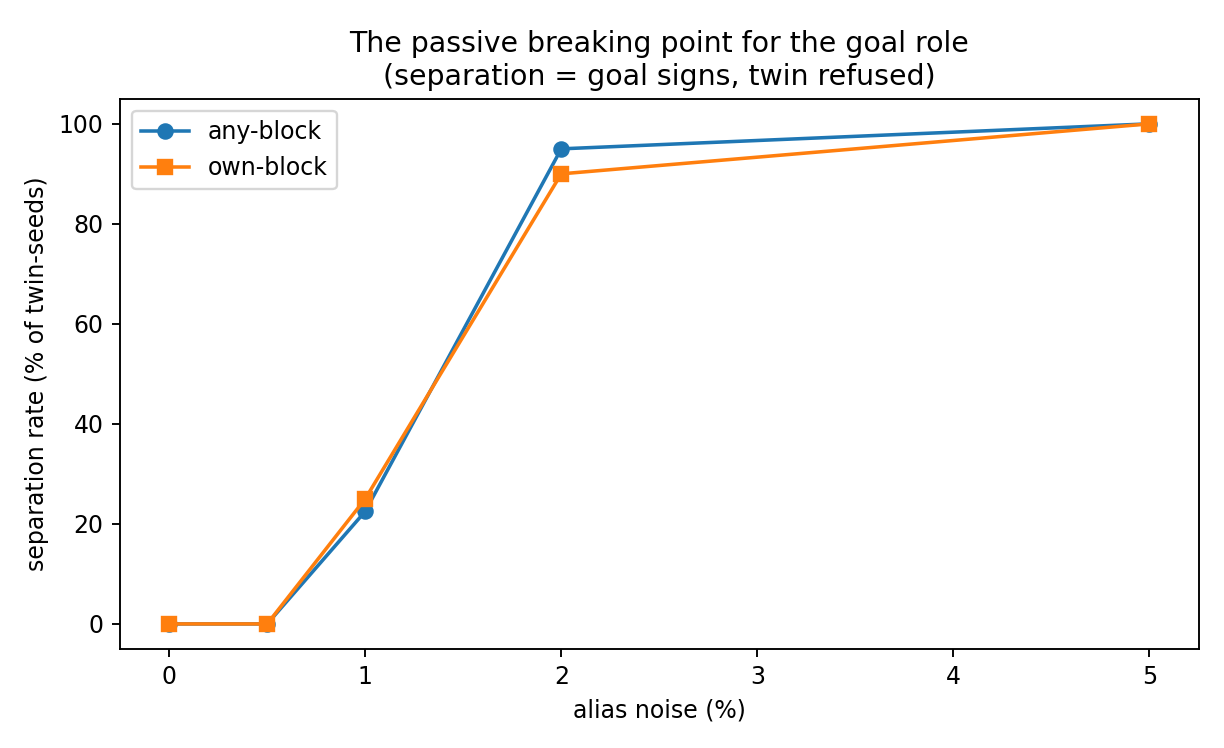
\includegraphics[width=0.62\linewidth]{fig_v3_zone_map.png}
\caption{Experiment 3: separation rate (goal exhibits the signature, twin does not)
versus twin noise --- the passive breaking point for the goal role lies between 1\% and
2\%.}
\label{fig:v3}
\end{figure}

\paragraph{The twin channel.}
In the alias no-core condition the \emph{disconnected} goals still exhibited the
signature in 20/20 seeds --- correctly: a goal stripped of its behavioural wiring still
causally drives its own recording, so ``drives without being driven'' genuinely holds
through the record. The instrument was right and the control's expectation was
mis-specified for twin-bearing worlds. Philosophically the point is sharp: a value can
persist in the signature through its records alone.

% =====================================================================
\section{Discussion}
% =====================================================================

\paragraph{What was established.}
The empowerment--plasticity signature locates a planted value structure from passive
observation, uniquely, across single- and multi-agent worlds, and refuses decoys,
disconnected goals, scrambles and (with the right conditioning) meters; the block-level
any-block convention is the only tested instrument whole at the scale of the UAD
authors' multi-agent simulator. Its limits are now measured rather than conjectured ---
history-triggered captured goals defeat lag-1 passivity; twins below $\approx 1$--$2\%$
noise are passively indistinguishable --- and interventional access closes exactly these
gaps, giving a quantitative form of the access-model thesis of \citet{zarncke2026uad}.
Several findings concern method rather than result: the XOR cipher; the self-penalising
floors; the collapse-detector role of the no-core control; and the value of running
disagreeing conventions in parallel rather than picking a primary early --- twice, the
convention we would have discarded first turned out to carry the mechanism.

\paragraph{Why structure, not behaviour.}
Behavioural inference and structural discovery are complementary, but structure has a
distinctive advantage under adversarial conditions: an agent that conceals its
objectives by adding decision noise weakens the behavioural signal, yet the component
that most drives behaviour beneath that noise remains structurally locatable; once
located, it can be isolated and studied in a regime where the noise no longer obscures
it. Our results are a first indication that such structural location is possible.

\paragraph{Limitations.}
(1)~\emph{Single-variable values.} The instrument scores individual variables. It has
been tested on agents with multiple belief states but not with multiple goal or value
states; a value structure distributed over several components is beyond it as it stands.
The grown-keys results suggest one route (deciphering interactions among several
value-like variables); we conjecture a better one --- use UAD's boundary-detection
machinery to identify sub-systems within an agent, then evaluate the empowerment and
plasticity of those sub-systems rather than of single variables. (2)~\emph{Lag-1
conditioning}, which the slow captured goal exploits; multi-horizon conditioning is the
evidenced remedy. (3)~\emph{Planted structure.} All worlds are engineered; whether the
polarisation \emph{emerges} in evolved or learned systems is the question the instrument
now makes askable, not one it has answered. (4)~The protocol was soft-blind: the
implementing system had read the world's source; protection came from the world's
independent origin, pre-registration, controls and multi-seed sweeps.
(5)~The relation between this signature and Omohundro's drives is a hypothesis
supported by recoverability, not a demonstration that empowered-and-stable components
\emph{function} as values in richer agents.

\paragraph{Future work.}
Systems-of-agents environments in which values may be held by coalitions rather than
individuals (any-block requires no assumption about which agent owns a value, and so
is structurally open to this); multi-horizon conditioning; sub-system-level scoring for
distributed value structures; and the twin channel as a probe of value persistence
through records.

% =====================================================================
\section*{Author contributions and disclosure}
% =====================================================================
S.B.\ conceived the hypothesis and framing, made all design decisions, reviewed every
audit and pre-registration in plain language, and directs the programme. Claude, an AI
system, wrote all code, ran the experiments and analyses, and drafted this manuscript
under S.B.'s direction; every decision, deviation and defect is dated in the project's
decisions log. \textbf{This manuscript is, as it stands, AI-generated} --- S.B.\ intends
to write the account in their own words when time allows --- and it is not being
submitted for publication.

\section*{Reproducibility}
All code (\pkg{value\_detect}), world generators, audits, locked pre-registrations,
verdict tables and figures are archived with fixed seeds; the UAD benchmark code is
imported unmodified. Sweeps ran on a single laptop (v1 $\approx 1$ h; v2 $\approx 12.5$
h; v3 $\approx 37.5$ h at four workers).

\bibliographystyle{plainnat}
\bibliography{references}

\end{document}
